\chapter*{Acknowledgements}
%\section*{Acknowledgements}
\addcontentsline{toc}{chapter}{Acknowledgements}

This thesis represents the work I have carried out as a PhD student under the supervision of Professor Jan H. Jensen in his group of Biocomputational Chemistry.
Thank you to all who have supported me during my work at the third floor of C-building at the H.C. Ørsteds Institute.
\\\\I would especially like to thank the following people:

\begin{itemize}
\item Thank you to my supervisor, Jan "Yoda" Jensen for introducing me to the
    exciting fields of quantum chemistry and biocomputational chemistry, teaching me everything I know (and more), for your patience, and the inspiration you bring to everyone around you.

\item Thank you to Jens Breinholt at Novo Nordisk for supporting me with my work -- I sincerely hope, that my work will very soon become practically useable. And thank you to the Novo Nordisk STAR PhD program for financial support, and for giving me the opportunity to carry out this study.

\item Thank you to all of our collaborators at the Biocenter, who always have been very supportive. Especially, Thomas Hamelryck (in the presence of whom everything is trivially solved using Bayes' theorm) for helping me out with Bayesian theory, your great ideas and more, Wouter Boomsma for being seemingly all-knowing in what concerns PHAISTOS and always being exceptionally helpful, Simon Olsson for helping out with the implementation of the Jeffrey's prior code, and Kresten Lindorff-Larsen for always being encouraging and sharing your knowledge in this field.

\item Thank you to my office mates, Casper Steinmann, Jimmy Kromann and Lars Bratholm, for the invaluable company, our office pranks, and endless number of energy drinks consumed, as well as the highly valuable scientific discussions we continue to share daily (not forgetting the virtual monster we've slayed).

Also thank you to those close colleagues who came by for coffee and friendly conversations; Jonas Elm, Jacob Lykkebo, Nini Reeler, Frederik Beyer (and many, many more!).

\item Thank you to everyone at the Department of Chemistry, especially Kurt V.~Mikkelsen, Stephan P.~A.~Sauer and Sten Rettrup for always being so helpful with everything from bureaucratic procedures, to coupled cluster theory, to derivation of the Slater-Kloster tables.

\item Thank you to all the students in the courses I've taught, and especially the very talented students who have carried out Master's, Bachelor's and various research projects under my supervision. Of those not already mentioned (and in no particular order): Maher Channir, Anders Larsen, Rie Nielsen, Christine Skibsted, Cecilie Lindholm.

\item Thank you to everyone I forgot to mention, including all the unnamed developers of the free, open source software I use in my daily work -- the Open Babel project in particular.

\end{itemize}
Lastly, an even bigger thanks goes to my IRL family and friends, whom I have been seeing much less than I should since I undertook my PhD studies. Thanks, everyone!
%\begin{figure}[h!]
%\centering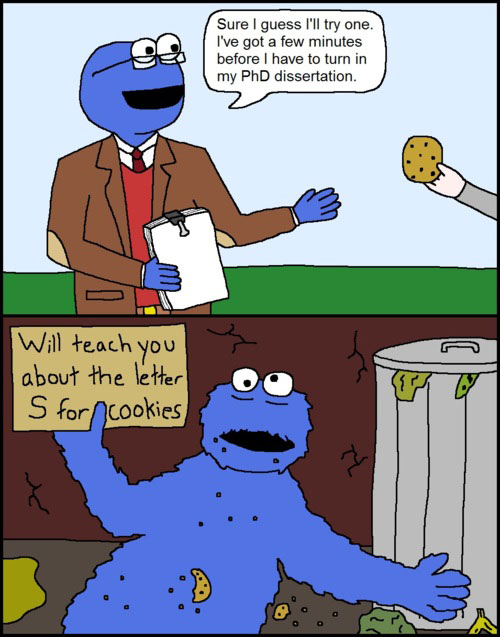
\includegraphics[width=0.6\textwidth]{figures/will-teach-you-about-the-letter-s-for-cookies.jpg}
%\end{figure}
\clearpage
\qquad
\vspace{15cm}
\subsubsection*{Licensing}
This work is published under the terms of the Creative Commons Attribution 4.0 International (CC-BY 4.0) license. See \url{http://creativecommons.org/licenses/by/4.0/} for the complete list of license terms.
This work, and all figures and scripts to compile them is available from \url{https://github.com/andersx/phd-thesis/}.
\begin{figure}[h!]
\centering
\includegraphics[width=0.4\textwidth]{figures/cc-by.pdf}
\end{figure}
